\documentclass[osajnl,twocolumn,showpacs,superscriptaddress,10pt]{revtex4-2}
%
%
\usepackage{dcolumn}% Align table columns on decimal point
\usepackage{bm}
\usepackage{bbm}
\usepackage{lipsum}
\usepackage[spanish,es-tabla]{babel}
\usepackage[utf8]{inputenc}
\usepackage[T1]{fontenc}
\usepackage{makeidx}
\usepackage{graphicx}
\usepackage{animate}
\usepackage{subfig}
\usepackage{gensymb}
\usepackage{physics}
\usepackage{amsmath}
\usepackage{amsfonts}
\usepackage{amssymb}
\usepackage{mathrsfs}
\usepackage[pdftex]{hyperref}
\usepackage{multirow}
\usepackage{float}
\usepackage{booktabs}
\usepackage{wrapfig}
\usepackage{minipage-marginpar}
\usepackage{boxedminipage}
\usepackage[dvipsnames]{xcolor}
%
\usepackage{fancyhdr}
\usepackage{fourier-orns}
%
\renewcommand{\headrule}{%
\vspace{2pt}\hrulefill
\raisebox{0pt}{\quad\decofourleft\decotwo\decofourright\quad}%
\hrulefill}
\setlength{\headheight}{35pt}
%
%
\AtBeginDocument{\selectlanguage{spanish}}
\decimalpoint
%\bibliographystyle{IEEEtran}
%\bibliography{IEEEabrv,mybibfile}
%
%
\begin{document}
%Titulo
%
%Comandos--------------------------------
\providecommand{\hs}[1]{\ensuremath{\hspace{#1 pt}}}
\providecommand{\hsn}[1]{\ensuremath{\hspace{#1 pt}}}
\providecommand{\vs}[1]{\ensuremath{\vspace{#1 pt}}}
\providecommand{\unitvec}[1]{\boldsymbol{\hat{#1}}}
\providecommand{\dif}[2]{ \ensuremath{\frac{d #1}{d #2}} }
\providecommand{\into}[2]{ \ensuremath{\oint_{#1}{#2}} }

\providecommand{\linft}[2]{ \ensuremath{\lim_{#1\rightarrow\infty}\corch{#2}} }

\providecommand{\parent}[1]{\ensuremath{\left(\hspace{2pt} #1 \hspace{2pt}\right)}}
\providecommand{\corch}[1]{\ensuremath{\left[\hspace{2pt} #1 \hspace{2pt}\right]}}
\providecommand{\llav}[1]{\ensuremath{\left\{\hspace{2pt} #1 \hspace{2pt}\right\}}}

\providecommand{\difn}[3]{ \ensuremath{\frac{d^{#3} #1}{d {#2}^{#3}}} }
\providecommand{\parti}[2]{ \ensuremath{\frac{\partial #1}{\partial #2}} }
\providecommand{\partin}[3]{ \ensuremath{\frac{{\partial}^{#3} #1}{{\partial} {#2}^{#3}}} }
\providecommand{\bs}[1]{\ensuremath{\boldsymbol{#1}}}

\providecommand{\pcruz}[2]{\ensuremath{ {#1}\times{#2} }}
\providecommand{\ppunt}[2]{\ensuremath{ {#1}\cdot{#2} }}
\providecommand{\bs}[1]{\ensuremath{ \boldsymbol{#1} }}

\providecommand{\llint}[4]{\ensuremath{\int_{#1}^{#2}\left\{\hsn{2} #3 \hsn{2}\right\}\hsn{1}{d{#4}} }}
\providecommand{\chint}[4]{\ensuremath{\int_{#1}^{#2}\left[\hsn{2} #3 \hsn{2}\right]\hsn{1}{d{#4}} }}
\providecommand{\print}[4]{\ensuremath{\int_{#1}^{#2}\left(\hsn{2} #3 \hsn{2}\right)\hsn{1}{d{#4}}}}
\providecommand{\clint}[3]{\ensuremath{\left[\hs{2} {#3} \hs{2}\right|_{#1}^{#2} }}
\providecommand{\inte}[4]{\ensuremath{ \int_{#1}^{#2}{#3}\hsn{1}{d{#4}} }}
\providecommand{\lne}[1]{\ensuremath{\ln{\left\{\hspace{1pt} #1 \hspace{1pt}\right\}}}}

\providecommand{\cose}[1]{\ensuremath{\cos{\left[\hspace{2pt} #1 \hspace{2pt}\right]}}}
\providecommand{\seno}[1]{\ensuremath{\sin{\left[\hspace{2pt} #1 \hspace{2pt}\right]}}}
\providecommand{\tang}[1]{\ensuremath{\tan{\left[\hspace{2pt} #1 \hspace{2pt}\right]}}}
\providecommand{\cota}[1]{\ensuremath{\cot{\left[\hspace{2pt} #1 \hspace{2pt}\right]}}}
\providecommand{\seca}[1]{\ensuremath{\sec{\left[\hspace{2pt} #1 \hspace{2pt}\right]}}}
\providecommand{\csec}[1]{\ensuremath{\csc{\left[\hspace{2pt} #1 \hspace{2pt}\right]}}}

\providecommand{\cosen}[2]{\ensuremath{\cos^{#2}{\left[\hspace{2pt} #1 \hspace{2pt}\right]}}}
\providecommand{\senon}[2]{\ensuremath{\sin^{#2}{\left[\hspace{2pt} #1 \hspace{2pt}\right]}}}
\providecommand{\tangn}[2]{\ensuremath{\tan^{#2}{\left[\hspace{2pt} #1 \hspace{2pt}\right]}}}
\providecommand{\cotan}[2]{\ensuremath{\cot^{#2}{\left[\hspace{2pt} #1 \hspace{2pt}\right]}}}
\providecommand{\secan}[2]{\ensuremath{\sec^{#2}{\left[\hspace{2pt} #1 \hspace{2pt}\right]}}}
\providecommand{\csecn}[2]{\ensuremath{\csc^{#2}{\left[\hspace{2pt} #1 \hspace{2pt}\right]}}}

\providecommand{\acose}[1]{\ensuremath{\cos^{-1}{\left[\hspace{2pt} #1 \hspace{2pt}\right]}}}
\providecommand{\aseno}[1]{\ensuremath{\sin^{-1}{\left[\hspace{2pt} #1 \hspace{2pt}\right]}}}
\providecommand{\atang}[1]{\ensuremath{\tan^{-1}{\left[\hspace{2pt} #1 \hspace{2pt}\right]}}}
\providecommand{\acota}[1]{\ensuremath{\cot^{-1}{\left[\hspace{2pt} #1 \hspace{2pt}\right]}}}
\providecommand{\aseca}[1]{\ensuremath{\sec^{-1}{\left[\hspace{2pt} #1 \hspace{2pt}\right]}}}
\providecommand{\acsec}[1]{\ensuremath{\csc^{-1}{\left[\hspace{2pt} #1 \hspace{2pt}\right]}}}

\providecommand{\sumat}[3]{\ensuremath{\sum_{#1}^{#2}{\left\{\hspace{2pt} #3 \hspace{2pt}\right\}}}}
\providecommand{\suma}[3]{\ensuremath{\sum_{#1}^{#2}{#3}}}
\providecommand{\Rarr}[1]{\ensuremath{\hs{#1}\Longrightarrow\hs{#1}}}
\providecommand{\rarr}[1]{\ensuremath{\hs{#1}\longrightarrow\hs{#1}}}

\providecommand{\expo}[1]{\ensuremath{e^{#1}}}
\providecommand{\uvec}[1]{\ensuremath{\hat{#1}}}

\title{La influencia de Genshin Impact en el mercado occidental (improvisado)}
\thanks{Laboratorio de reducción de datos}

\author{Mario Armando, Urbina Silva}\email{mariosva139@gmail.com}
\affiliation{Escuela de Ciencias Físicas y Matemáticas, Universidad de San Carlos de Guatemala, Ciudad Universitaria, Zona 12, Guatemala.
}%
%\affiliation{}
%\collaboration{MUSO Collaboration}%\noaffiliation
%\date{\today}%
%Resumen
\begin{abstract}
    Hola
\end{abstract}
\maketitle
\section{Introducción}
Los videojuegos se han ido introduciendo cada vez más en la sociedad de hoy en día. Al inicio de los años 90, el videojuego se convirtiò en algo que iba adquiriendo forma con el pasar del tiempo, dejó de ser solamente entretenimiento puro, empezó a contar grandes historias, mejores que muchas de las películas del momento, convirtiendo de esta forma a la industria del videojuego en un importante sector económico. Con la entrada de los años 2000 fue el comienzo de la modalidad online de diversos títulos que causaron gran furor en su momento, y a la vez que algo se hace popular, resulta mucho más sencillo sacar probecho de ello.
\\\\
A partir de ello, la industria de los videojuegos se fue consolidando a nivel económico, uniéndose a colosos como la música, el cine y la televisión, y con ello tras la mitad de la década del 2010 dicha industria llegó a facturar más dinero que el cine y la música juntos\cite{ONTSI}. Entre muchas cosas negativas, de esta industría, se puede mencionar que con la creación de los videojuegos surgió la adicción a estos y el tiempo que los jugadores dedicaban a ellos. Dicho problema se ha ido agravando con el paso de los años, y no solamente con los juegos en sí; sino que ha empeorado con la popularización de los juegos gacha, juegos gratuitos con micro transacciones que han estado en el punto de mira por su similitud a las máquinas trapaperras y demás elementos encontrados en casinos, con la diferencia de que los juegos gacha son totalmente gratuitos\cite{Navarro}.
\\\\
Con el avance de la tecnología se tiene hoy en día que cualquier aficionado a los videojuegos pueda encontrar su estilo de juego preferido y disfrutar dicho medio de entretenimiento durante horas. Gracias a las plataformas móviles, los denominados juegos \textit{gacha}, género que en el pasado estuvo limitado a una pequeña base de fans, están cobrando cada vez mas popularidad a nivel mundial.
\\\\
Los juegos gacha son videojuegos que animan a los jugadores a utilizar su propia modena interna para comprar artículos virtuales mientras progresan en la partida. Estos juegos permiten ganar artículos como cartas y personajes a través de un mecanismo muy similar al de las maquinas expendedoras girando una ruleta o realizando una tirada de datos mediante la moneda del juego para obtener un artículo aleatorio. \cite{gacha}
\\\\
Los juegos gacha se han convertido en un gran modelo de negocios en los últimos años, estos empezaron ganando popularidad en Asia, y ahora con la opción portatil, siguen sumando fanáticos de los juegos para móviles en todo el mundo. Este género ha ganado reputación sobre la base de la incertidumbre, esto se debe a que con ofertas de recompensas sorpresa y sus tramas en constante evolución, los videojuegos gacha han estado cautivando a jugadores de todas las tendencias desde 2010. \cite{gacha02}

\section{Definición de un videojuego gacha}
El término gacha proviene de las máquinas dispensadoras japonesas denominadas Gashapón. Su nombre viene de una combinación de diferentes onomatopeyas, la primera parte definiría el sonido de la máquina dispensadora (gasha-gasha) y la segunda parte sería el sonido del objeto saliendo de la máquina (pon). El funcionamiento del gacha es muy sencillo. En primer lugar, se introduce en dinero en la máquina, se gira una manivela o se tira de una palanca y se obtiene una bola de plástico que contiene el objeto que nos ha tocado. Al acto de pagar para obtener un objeto de este tipo de máquinas se le denomina pullear o rollear, que traducido significa tirar y rodar respectivamente, ya que representan la acción de tirar de la palanca (pull) o la acción de hacer girar el mecanismo (roll). Estos términos se utilizan tanto en inglés como en castellano.
\\\\
Al momento de introducir dicho concepto en el mundo de los videojuegos, los desarrolladores vieron en dicho sistema de recompensa un modelo de negocio, especialmente para los videojuegos móviles gratuitos, de manera que desde el 2012 dicho sistema empezó a popularizarse. En general, los videojuegos gacha no se centran en su jugabilidad, la cual suele ser bastante simple al principio y poco a poco se va complicando para mantener a sus jugadores activos, entretenidos y conseguir atraer nuevos usuarios, sino en la obtención de recursos, ya sean personajes, armas, trajes, equipamiento y demás. Para obtener dichos elementos normalmente se realiza una tirada a una máquina sin límite siempre y cuando se tenga la moneda que pide el juego para hacerlo. Estas imitaciones de las máquinas reales han de establecer unas probabilidades para obtener objetos, de forma que, a mayor rareza, menor probabilidad habrá de obtener el objeto.\cite{Navarro}
\\\\
El método de pago es relativamente sencillo, se canjea la moneda del juego por una tirada, y mediante una animación se revela la rareza y el objeto obtenido. Una vez finalizada la tirada de gacha, ya se podrá usar el objeto obtenido sin limitación alguna. Los juegos gacha contienen una gran variedad de características las cuales se pueden dividir de la siguiente manera
\begin{table}[H]
    \begin{center}
        \begin{tabular}{|ccc|} \hline
            \multicolumn{3}{|c|}{Juegos Gacha}                            \\ \hline
            \multicolumn{1}{|c|}{\textbf{Tipos}} & \multicolumn{1}{c|}{\textbf{Géneros}} & \textbf{Mecánicas relacionadas} \\ \hline\hline
            \multicolumn{1}{|c|}{\begin{tabular}[c]{@{}c@{}}Gacha\\ completa\end{tabular}} & \multicolumn{1}{c|}{\begin{tabular}[c]{@{}c@{}}Juegos de\\ estrategia\\ por turnos\end{tabular}} &  \\ \hline
            \multicolumn{1}{|c|}{\begin{tabular}[c]{@{}c@{}}Caja\\Gacha\end{tabular}} & \multicolumn{1}{c|}{\begin{tabular}[c]{@{}c@{}}Juegos\\ inactivos o\\ IDLE\end{tabular}} & Banners \\ \hline
            \multicolumn{1}{|c|}{\begin{tabular}[c]{@{}c@{}}Gacha\\ sugoroku\end{tabular}} & \multicolumn{1}{c|}{Juegos rítmicos} & Objetos de preferencia \\ \hline
            \multicolumn{1}{|c|}{\begin{tabular}[c]{@{}c@{}}Gacha con\\ reintento\end{tabular}} & \multicolumn{1}{c|}{} & Pity Break System \\ \hline
            \multicolumn{1}{|c|}{\begin{tabular}[c]{@{}c@{}}Gacha\\ consecutivo\end{tabular}} & \multicolumn{1}{c|}{} & Spark System \\ \hline
            \multicolumn{1}{|c|}{\begin{tabular}[c]{@{}c@{}}Gacha\\ intensificado\end{tabular}} & \multicolumn{1}{c|}{} & Objetos duplicados \\ \hline
            \multicolumn{1}{|c|}{\begin{tabular}[c]{@{}c@{}}Gacha\\ abierto/cerrado\end{tabular}} & \multicolumn{1}{c|}{} & PvP \\ \hline
            \multicolumn{1}{|c|}{\begin{tabular}[c]{@{}c@{}}Gacha con\\ descuento\end{tabular}} & \multicolumn{1}{c|}{} & Eventos \\ \hline
        \end{tabular}
        \vs{-5}
        \caption{\label{Res-mec-gatcha}Resumen de las mecánicas de los juegos gatcha, Navarro 2021 \cite{Navarro}}
    \end{center}
\end{table}
\section{Genshin Impact}
Genshin Impact es un juego de rol de acción de mundo abierto desarrollado por miHoYo que nos lleva hasta Teyvat, un mundo de fantasía donde los siete elementos fluyen y convergen. En el rol de un viajero de otro mundo recién despertado en esta tierra, el jugador tiene la misión de buscar a Los Arcontes de los Siete Elementos, unos seres mortales. Cada pasaje de la aventura de Genshin Impact desenterrará algo milagroso, y lo perdido será finalmente encontrado.
\\\\
Genshin Impact se hace fuerte en su ambientación, con cierto parecido al vasto mundo de Hyrule creado por Nintendo para The Legend of Zelda: Breath of the Wild pero con suficiente fuerza e identidad propia como para ofrecer al jugador una experiencia visual totalmente inmersiva.\cite{3DJuegos} Dicha similitud es uno de los aspectos más criticados del juego, aunque finalmente 'Genshin Impact' ha sobrevolado un poco esta polémica y ha terminado adquiriendo una fama por derecho propio. Al fin y al cabo, elementos como la necesidad de cocinar, los campamentos enemigos que rapiñar, el medidor de estamina o las torres que permiten viajar de un punto a otro del mapa con rapidez no las inventó Nintendo\cite{xataka}. En ese objetivo sus responsables garantizan paisajes majestuosos, animaciones desbordantes en tiempo real y movimientos de personajes finamente detallados así como un sistema de iluminación y tiempo que cambia conforme se avanza en la partida, todo rodeado por una cuidada banda sonora.
\\\\
miHoYo también apuesta su capital a un sistema de combate elemental. Su funcionamiento parte de la premisa de dominar los siete elementos de su mundo—Anemo, Electro, Hydro, Pyro, Cryo, Dendro y Geo— para desencadenar diferentes reacciones. Por otra parte, quienes deseen llegar lo más lejos posible en el videojuego se han de armar un poderoso equipo, escogiendo entre una amplia selección de personajes, cada uno con personalidades, historias y habilidades únicas.
\\\\
Genshin Impact es uno de los grandes éxitos free-to-play del 2020 para PC, PS5, PS4 y móviles iOS y Android, y un referente de la nueva hornada de títulos desarrollados en China para Occidente\cite{3DJuegos}.

    \subsection{El gancho del gacha}
    Hay un concepto en el juego, que es el del "world level", que limita el nivel al que puede llegar el jugador, las misiones que puede aceptar y otros aspectos que claramente impiden definir 'Genshin Impact' como un sandbox al uso. Así que mientras ese "world level" se incrementa y permite realizar más acciones, hay que aceptar misiones y vagabundear por el mundo subiendo poco a poco de nivel. En ocasiones, muy poco a poco.
    \\\\
    Detrás de esta mecánica, por supuesto, hay truco. 'Genshin Impact' es un gacha, un subgénero habitual en los free-to-play en el que los jugadores acceden a mejoras a través de máquinas que dan premios de forma arbitraria, al estilo de las polémicas e infaustas loot boxes. Por supuesto, estas máquinas funcionan con dinero real, y es una mecánica lógicamente criticada que se ha adueñado del panorama móvil chino y coreano. 'Genshin Impact' es uno de los primeros juegos masivos en popularizar la mecánica en occidente.
    \\\\
    En el caso de 'Genshin Impact', y posiblemente de ahí viene su popularidad y la moderada buena fama que tiene entre jugadores tradicionales, las mecánicas gacha no son especialmente intrusivas y solo se acentúan al final.
    \\\\ 
    También en este aspecto de usar técnicas poco tradicionales para atrapar al jugador, 'Genshin Impact' se revela maquiavélico a partir del nivel 20, donde hay que subir equipo y personaje con recursos difíciles de conseguir, lo que introduce en la ecuación a los Dominios, mazmorras que otorgan recompensas según el día de la semana que sea. Es decir, el juego de miHoYo presiona al jugador para que acceda a las partidas a diario, generando esa necesidad de volver una y otra vez a la exploración y la batalla.
    \\\\
    Cómo todo eso ha confluido en un juego coherente y que el jugador no percibe como un enganchapardillos es el auténtico milagro de 'Genshin Impact'. Jugadores y analistas están pasmados de que un free-to-play sea capaz de brindar al jugador un mundo de tamaño muy superior a lo habitual, con unas mecánicas más trabajadas (aquí solo hemos sobrevolado sobre ellas en términos generales, ya que como en todo RPG hay decenas de factores que manejar para mejorar los stats) y que no se explora simplemente pateando descampados, sino que hay que poner en marcha y mejorar poderes, e ingeniárselas a base de escalada, vuelo y localización de accesos secretos para husmear a fondo el terreno\cite{xataka}.

\section{Metodología}
Los datos acerca de las ingresos por mes, desde la salida del juego, en la región de occidente, incluyendo japón, se recolectaron del documento subido por J. Clement en  la página de Statista. Del mismo modo, se recolectaron datos de la página GachaRevenue, sin embargo estos comenzaban desde diciembre del 2022; y para los datos de los diferentes banner, desde la salida hasta el 20 de febrero del 2024, se recolectaron de la página de GENSHINLAB. Los parámetros utilizados para el presente estudio fueron el número de mes y los ingresos que obtuvo la empresa de miHoYo en dicho mes (dichos datos no incluyen las ventas de todas las plataformas).
\\\\
Para determinar si el ingreso económico, por mes, es consistente con algun tipo de distribución se decidió usar el logaritmo de dichos datos, dado que el hecho de utilizar los valores originales podría afectar el ajuste/fit con respecto a los datos, presentando de esta forma grandes inconsistencias en el ajuste. Por lo tanto, para demostrar dichos diferencias se realizó el análisis de los datos tanto en su forma original como en su forma logarímica.
\\\\
Es por ello que se procedió a determinar la matriz de covarianza, para determinar la dependencia entre los ingresos a lo largo del tiempo (en este caso se analiza respectivamente los ingresos mensuales); así mismo, se determinaron los coeficientes de correlación de Pearson, Spearman y el coeficiente de correlación de rango de Kendall para analizar de mejor manera los datos y determinar de esta forma si los datos tienen correlación alguna.
\\\\
Por último, empleando el programa de GnuPlot y Python, utilizando las librerías de pandas, mpmath y scipy.stats, se realizarón las gráficas de los datos de ventas por mes y ventas por banner de personaje, realizando diferentes tipos de curvas para ver cual se ajustaba de mejor manera a los datos y de esta forma se pudiera predecir de cierta forma los ingresos de miHoYo, tanto por parte de occidente como en el caso del banner que representan los ingresos por parte de la iOS de China (sin incluir ordenadores PC).

\section{Resultados}
Como ha de saberse, a la hora de calcular datos de ventas hay que tomar en consideración la acogida que tiene dicho producto en el mercado, más aun cuando se trata de ventas de un juego cacha en donde el "hype" por cierta cosa, personaje, skin puede influir a que la comunidad pague más para obtener dicho producto o no; además, también hay que tomar en consideración la influencia que tienen los creadores de contenido en la comunidad de jugadores y en algunas ocasiones sobre las decisiones de algunos jugadores. Es por ello que los datos a analizar no tienen una distribución que las represente de manera fiable y en su mayoría se analizaran las curvas de ajuste con respecto a los posibles ingresos de ventas que pueda tener el juego de Genshin Impact a un pequeño plazo.
\begin{figure}[H]
    \begin{center}
        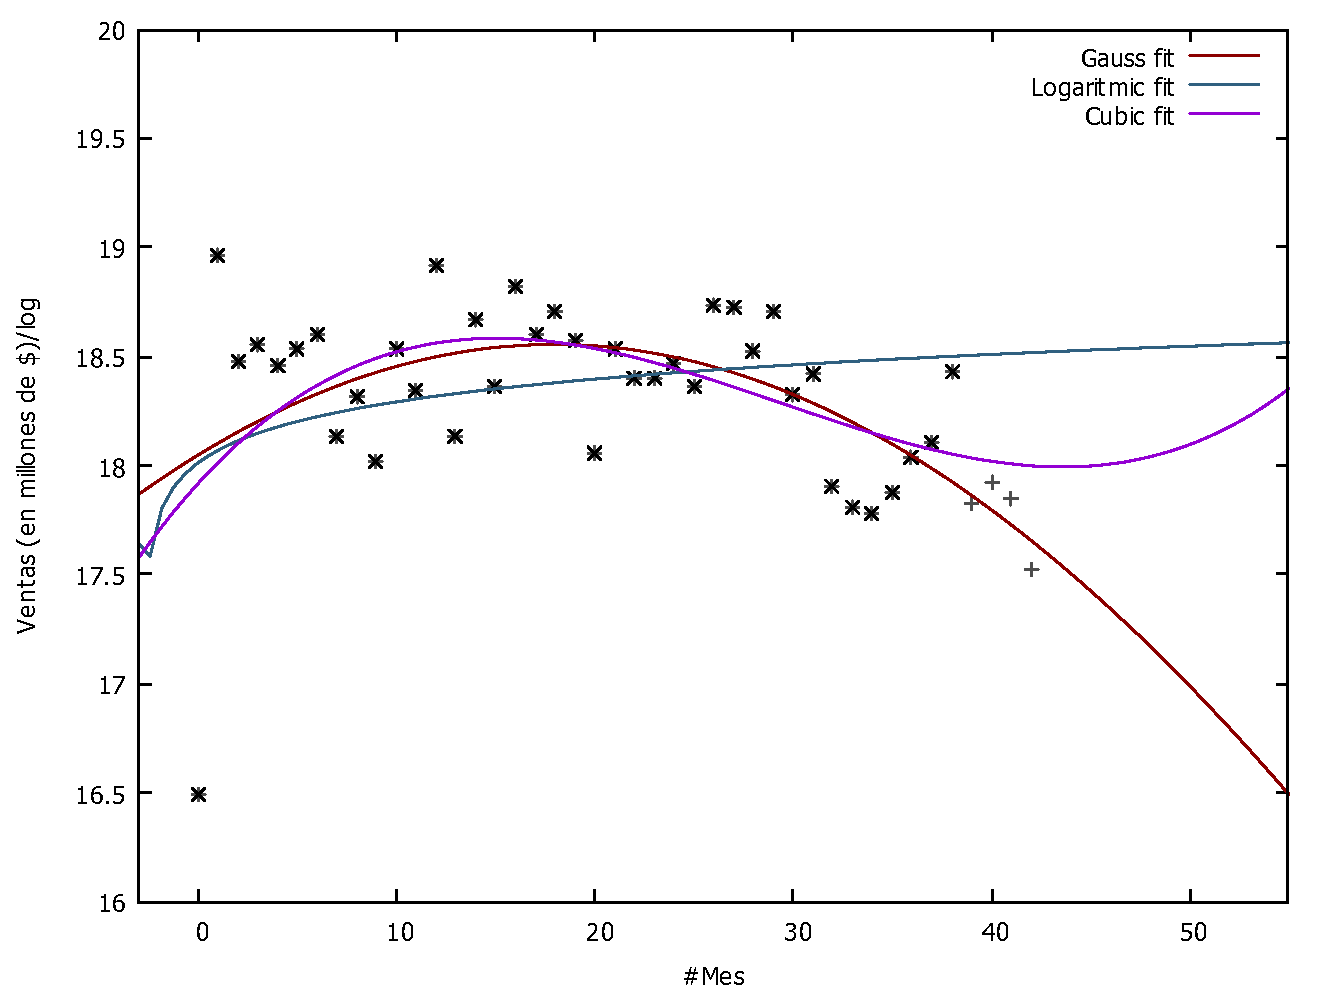
\includegraphics[width=0.4\textwidth]{img/GIRev01.pdf}
        \caption{\label{G01-statista}Ingresos por mes (base logarítmica), Statista 2024}
    \end{center}
\end{figure}
Como se puede observar en la figura \ref{G01-statista}, donde se tienen datos desde septiembre del 2020 (mes en el que salió Genshin Impact), la curva de ajuste cúbica puede ser una de las mejores predicciones dado que comenzando el mes de abril recién habia salido un nuevo personaje por la comunidad del juego (Chiori), irónicamente muy poco bien recibido, de igual manera se puede observar en el penúltimo dato presentado en la figura \ref{G02-GachaRevenue}; sin embargo, no sería hasta finales del mes de abril e inicios del mes de mayo fuese a haber aumento en los igresos debido al nuevo personaje, uno de los más esperados desde la presentación del mismo en uno de los tantos avances de la trama. Esto último se podría corroborar observando la tendencia del último dato de la gráfica \ref{G02-GachaRevenue}, que de cierta forma su valor se acerca a la curva de ajuste cúbica de la figura \ref{G01-statista}.
\begin{figure}[H]
    \begin{center}
        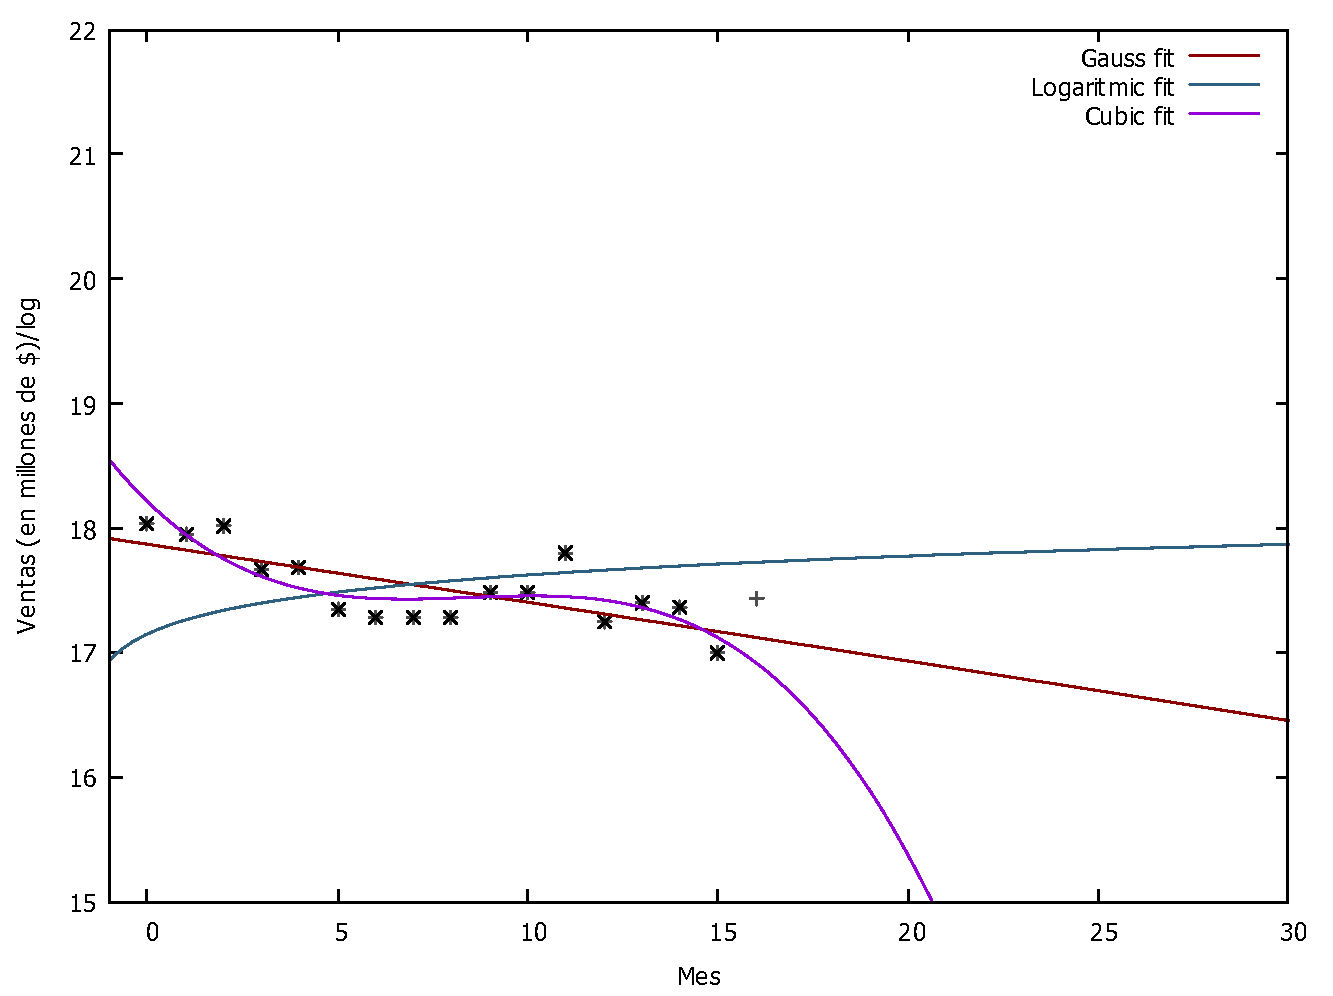
\includegraphics[width=0.4\textwidth]{img/GIRev02.pdf}
        \caption{\label{G02-GachaRevenue}Ingresos por mes (base logarítmica), GachaRevenue}
    \end{center}
\end{figure}
De esta forma se puede determinar que las curvas de ajuste, tanto de la distribución de gauss, logarítmica y cúbica, que se pueden observar en la figura \ref{G02-GachaRevenue} no se acoplan a lo esperado y con ellas no se puede observar un panorama aceptable de ventas a corto plazo. Esto se debe a que las funciones de distribución de gauss y cúbica indican una gran caída de ventas, lo cual, al observar los datos de ventas en la gráfica \ref{G01-statista}, no tiene ningún sentido. Del mismo modo se descarta la posibilidad de la función logarítmica debido a que las ventas del mes de mayo, con la entrada de la segunda mitad de la versión y cambio de banner, no se vislumbran tan altas como indica la curva de ajuste logarítmica.
\begin{figure}[H]
    \begin{center}
        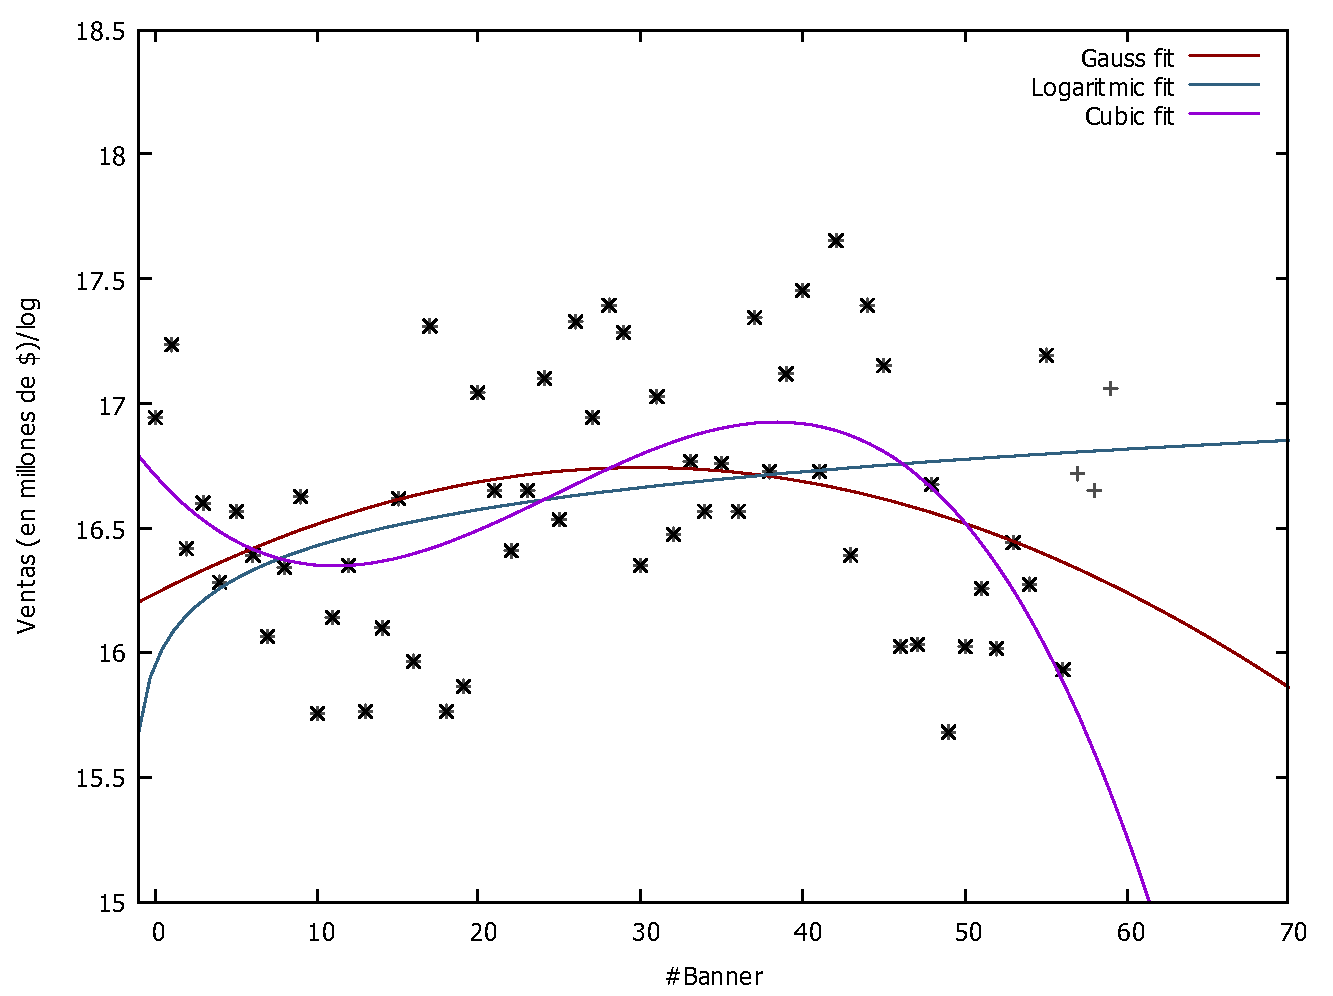
\includegraphics[width=0.4\textwidth]{img/GIBannChRev02.pdf}
        \caption{\label{G03-iOS}Ingresos por banner iOS China (base logarítmica), ajuste omitiendo datos, GenshinLab}
    \end{center}
\end{figure}

\begin{figure}[H]
    \begin{center}
        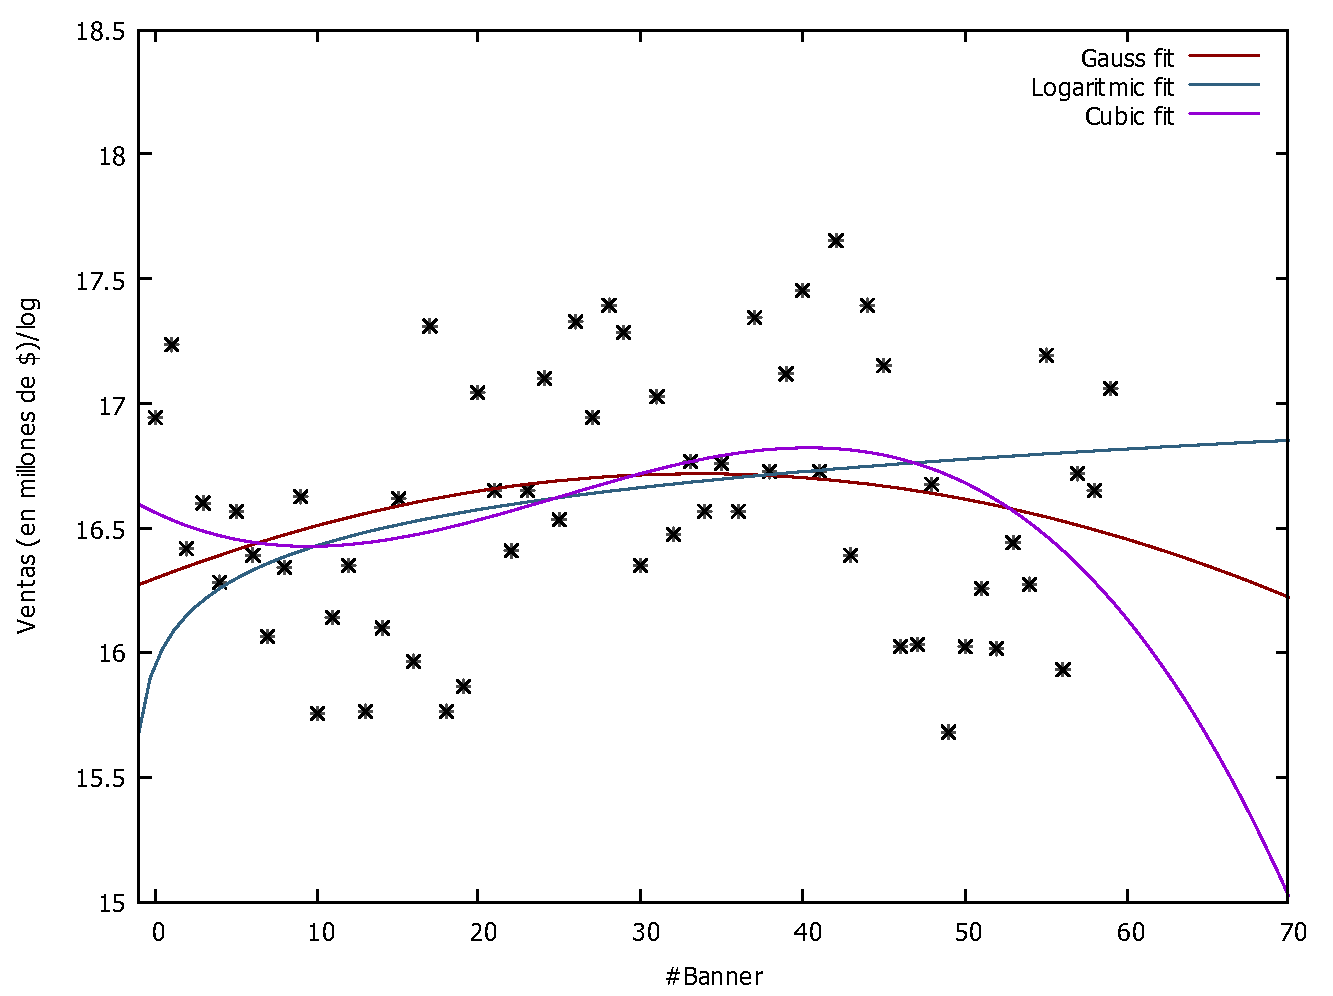
\includegraphics[width=0.4\textwidth]{img/GIBannChRev01.pdf}
        \caption{\label{G04-iOS}Ajuste de ingresos por banner iOS China (base logarítmica), GenshinLab}
    \end{center}
\end{figure}

\section{Conclusiones}
    \begin{itemize}
        \item El rozamiento viscoso se da como consecuencia de la fricción que presenta un fluido respecto a un objeto.
        \item La ley de Poiseuille se cumple fluidos con viscosidad constante, es decir, en fluidos homogéneos.
        \item El número de Reynolds favorece los flujos turbulentos, como consecuencia de la aceleración y desaceleración del pulso, en el caso del flujo sanguíneo.
    \end{itemize}

    \nocite{*}
    \bibliography{ref.bib}
\end{document}